\chapter{Software and Set-up}
\label{chap:software}
\section{Downloading BioPype}
%
\begin{enumerate}
\item Go to the BioPype Github repository at \url{https://github.com/EthanGniot/BioPype}. It should bring you to a page that looks like \ref{fig:biopype-github}.

\item Click on the green "Clone or download" button (see Figure \ref{fig:biopype-github})
    \begin{itemize}
    \item \small Note: The Github page that the URL from step 1 brings you to contains the code for the most recent "master" update to the BioPype repository. The "master" updates are usually the most recent \textit{stable} versions of BioPype. However, there may also be other versions of BioPype that are newer, but may contain bugs due to being under active development. To access these versions, click on the "branches" link (in Figure \ref{fig:biopype-github}, it is the link that says "4 branches" next to a branching symbol). If there are any branches (i.e., "versions") of BioPype that are more-current than the "master" branch, you will be able to see them on this page. This page also has links to the branches, where you can download that version of the BioPype code.
    \end{itemize}
%
    \begin{figure}[hbtp]
        \begin{maxipage}
        \hrule
        \centering
        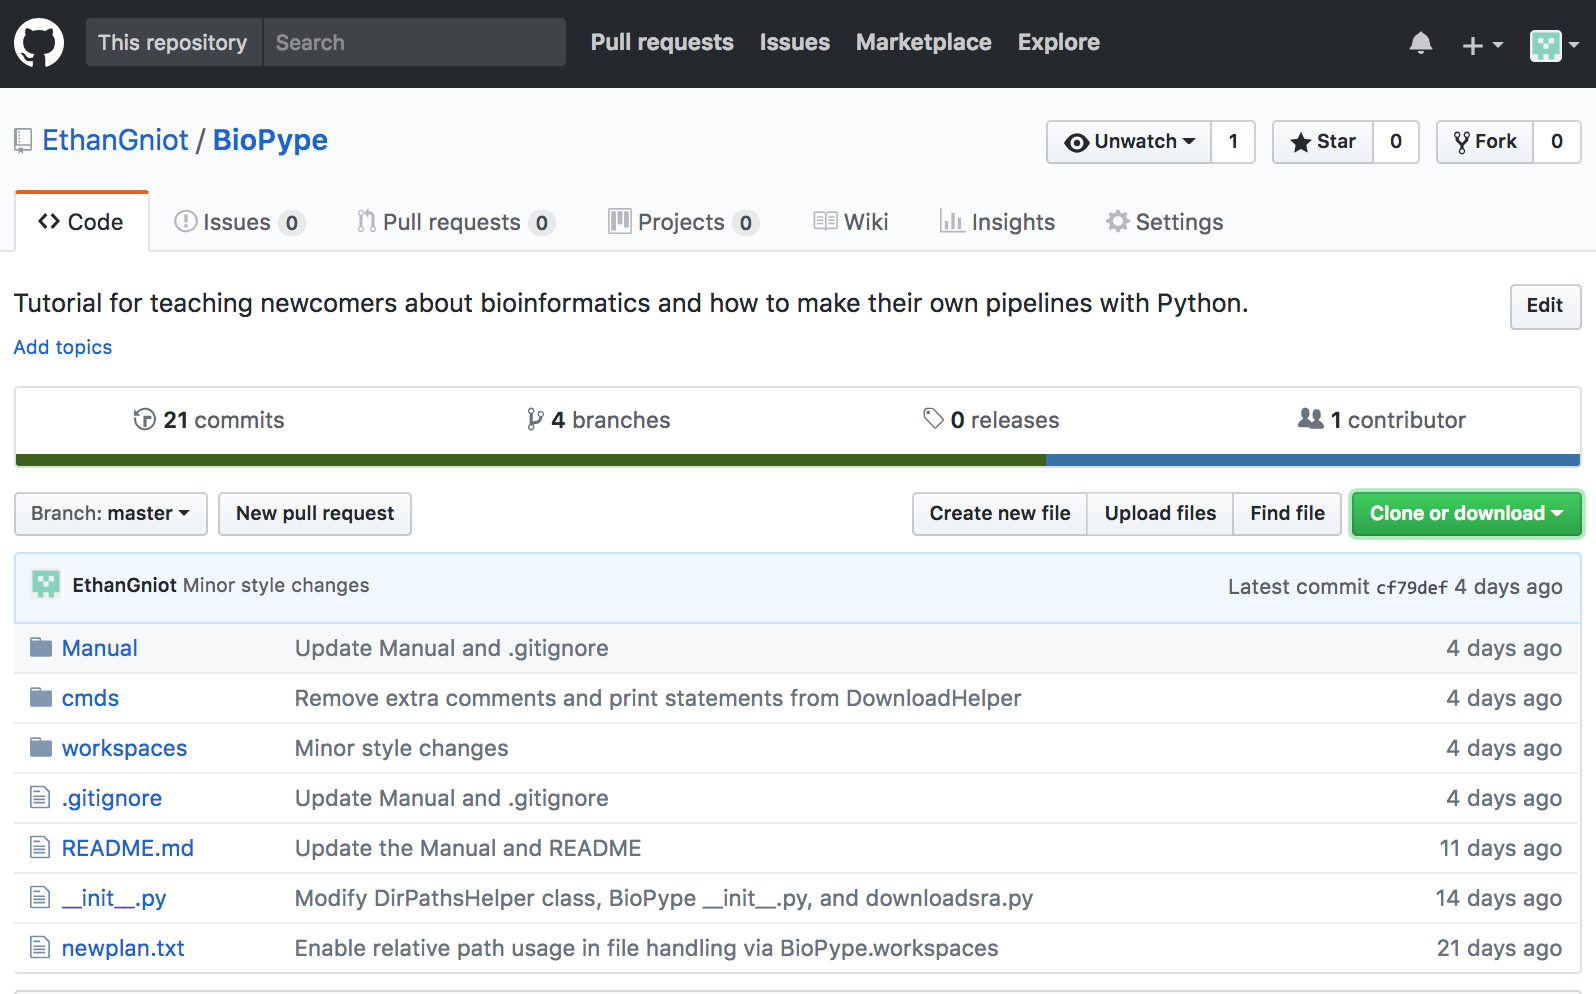
\includegraphics[height=8.5cm, width=13cm]{biopype-github}
        \caption{The BioPype Github webpage.}
        \label{fig:biopype-github}
        \hrule
        \end{maxipage}
    \end{figure}


\item Click on the "Download ZIP" button (the blue button in Figure \ref{fig:biopype-download}).
    \begin{figure}[hbtp]
        \begin{maxipage}
        \hrule
        \centering
        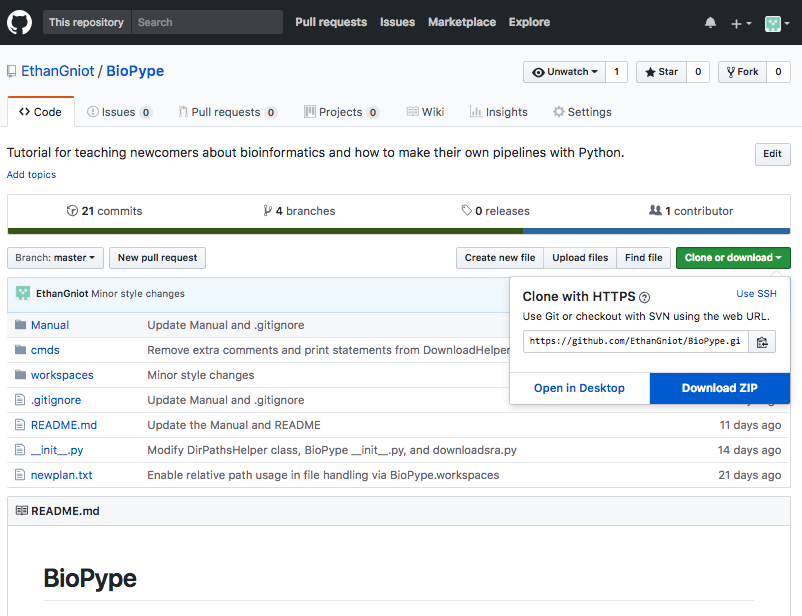
\includegraphics[height=8.5cm, width=13cm]{biopype-download}
        \caption{The button to download the BioPype code repository as a .zip file.}
        \label{fig:biopype-download}
        \hrule
        \end{maxipage}
    \end{figure}
    

\item Navigate to your Downloads folder and unzip the BioPype .zip file. 
    
\end{enumerate}

%
\section{BioPype Dependencies Information}
The following tables contain 

\verb|conda create -n test2 --file spec-file.txt|

%
\begin{table}[hbtp]
    \begin{maxipage}
    \caption{\textbf{Python packages that BioPype requires in order to function.}}
    \hrule
    \begin{tabular}{ l | l | l l }
        \textit{Package name} & \textit{Version number} & \textit{Command-line install} \\ 
        \hline
        Anaconda & 5.1 &  \\  
        multiqc & 1.5 & \verb|conda install -c bioconda multiqc| \\
        pandas & 0.22.0 & \verb|conda install pandas| \\
        parallel-fastq-dump & 0.6.3 & \verb|conda install -c bioconda parallel-fastq-dump| \\
        qiime2 & 2018.4 & (see above) \\
        sra-tools & 2.8.2 & \verb|conda install -c bioconda sra-tools| \\
        trim-galore & 0.4.5 & \verb|conda install -c bioconda trim-galore| & \\
    \end{tabular}
    \label{tab:software}
    \label{software}
    \hrule
    \end{maxipage}
\end{table}
%
\begin{table}[hbtp]
\begin{maxipage}
\caption{\textbf{Links to the documentation pages for BioPype's dependencies.}}
\begin{tabular}{ l | p{12.25cm} }
\textit{Software name} & \textit{Documentation link} \\
\hline
Anaconda & \url{https://docs.anaconda.com/anaconda/} \newline \url{https://conda.io/docs/user-guide/getting-started.html} \\
multiqc & \url{http://multiqc.info/} \\
pandas & \url{https://pandas.pydata.org/pandas-docs/stable/install.html} \\
parallel-fastq-dump & \url{https://github.com/rvalieris/parallel-fastq-dump} \\
qiime2 & \url{https://docs.qiime2.org/2018.4/} \\
sra-tools & \url{https://trace.ncbi.nlm.nih.gov/Traces/sra/sra.cgi?view=toolkit_doc} \\
trim-galore &  \url{https://github.com/FelixKrueger/TrimGalore} \\
\end{tabular}
\label{tab:software-doc-links}
\hrule
\end{maxipage}
\end{table}%



%
\section{Set-up and Install Dependencies}
Before we write any code, there are several steps that must be completed to prep your machine for the tasks we will be performing in this tutorial. Without these prerequisites, the code you write during this tutorial will not work correctly, and you won't be able to make use of BioPype:
\begin{enumerate}
\item Install and open Anaconda
\item Create a new virtual environment
\item Install packages
\end{enumerate}

\subsection{Install Anaconda or Miniconda}
\marginlabel{\footnotesize \textbf{Package manager:} (from Wikipedia) a collection of software tools that automates the process of installing, upgrading, configuring, and removing computer programs for a computer's operating system in a consistent manner}
As you can see in Table \ref{fig:software}, there are several packages that BioPype needs in order to function. Manually downloading and installing packages is an incredible pain, because the quirks of one package frequently conflict with quirks of another. To download the dependencies we need, we will use what's called a \textbf{package manager}. Essentially, package managers make it easy to install lots of packages because they can (usually) handle all of the minute details of the process, adjusting the versions and dependencies of each package to resolve any conflicts that would normally wreck the installation.

The package manager that we will be using is called \textit{conda}. There are two ways to obtain conda: the Anaconda distribution, and the Miniconda distribution.

\ul{Anaconda} is a set of about a hundred packages (many of which are useful scientific computing tools) that also comes bundled with a version of Python. One of these packages is the \textbf{conda} package (yes, conda is both a package and a package manager). One of the benefits of Anaconda is that it comes with a graphical interface for downloading and managing new packages called the Anaconda Navigator (see Figures \ref{anaconda-nav-win} and \ref{anaconda-env-win}). Conda can also be used to manage packages from a command-line interface (on a Mac, this is the Terminal application). However, the fact that Anaconda comes with over 100 packages pre-installed can sometimes cause problems when installing new packages. For that reason, you may choose to download Miniconda instead.

\ul{Miniconda} is a smaller alternative to Anaconda that is \textit{just} conda and its dependencies (as opposed to Anaconda, which is conda and a bunch of other packages). This means that Miniconda doesn't come with a graphical interface like the Anaconda Navigator, so conda must be operated from the command-line. However, it also means that Miniconda requires less storage on your computer (400 MB vs 3 GB) and also avoids some of the difficulties that come from Anaconda's pre-installed packages. 

We will cover two methods by which you can download the dependencies for BioPype using conda, one method uses the command-line with a Miniconda installation (faster, command-line only), and the other uses the Anaconda Navigator with an Anaconda installation (slower, standard graphical interface). 
\begin{itemize}
\item \attention{For the record, the command-line method should theoretically work just as well with an Anaconda installation as it does with a Miniconda installation, but I experienced unknown technical difficulties when trying to download all the dependencies with an Anaconda installation. Due to the unique file-state of individual machines, your mileage may vary.} 
\end{itemize}

\subsection*{Installing dependencies with Miniconda}
\begin{enumerate}
\item Go to \url{https://conda.io/docs/user-guide/install/index.html#regular-installation}, select your operating system, then follow the instructions to install Miniconda.


\item Once the installation is finished, 

\end{enumerate}



\textbf{\underline{Install and Open:}}

\begin{enumerate}
    \item Go to the download page for the Anaconda distribution at \\ \url{https://www.anaconda.com/download}. 
    \item Select your preferred operating system from the Windows, macOS, or Linux tabs, then select the Download option for the \textbf{Python 3.6 version} (Figure \ref{anaconda_download}) and follow the installation instructions.
    %
    \begin{figure}[h]
        \begin{center}
        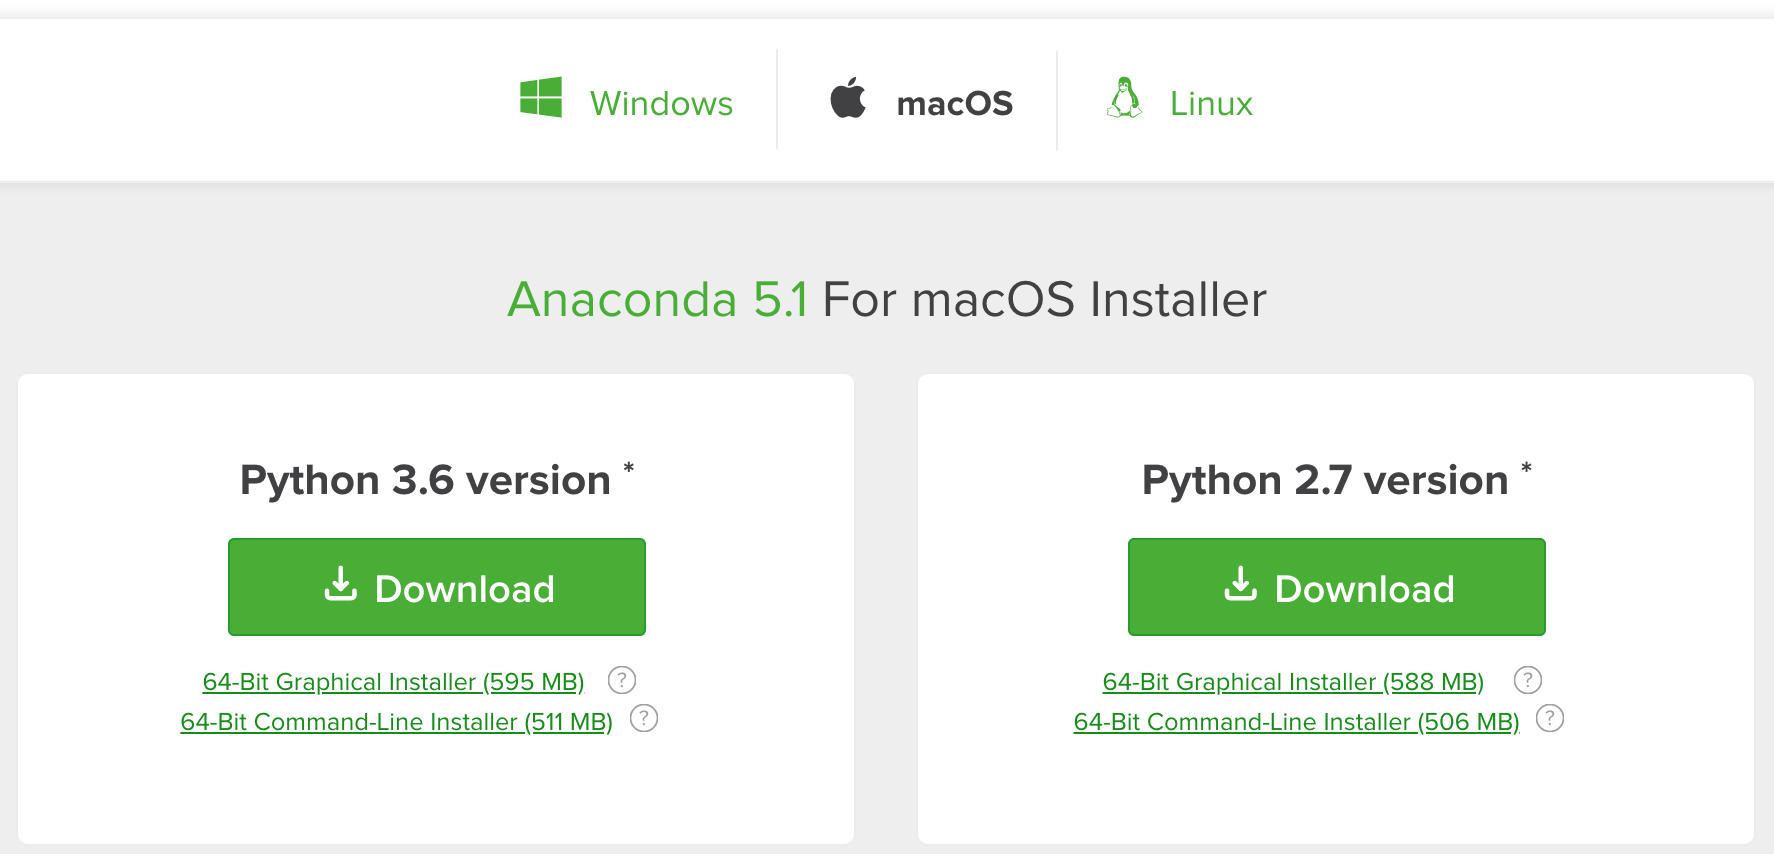
\includegraphics[width=9.5cm]{anaconda_download}
        \caption{The Anaconda download options provided on the Anaconda distribution website at \protect \url{https://www.anaconda.com/download}}.
        \label{anaconda_download}
        \end{center}
    \end{figure}
    %


    \item After installation is complete, open the application named "Anaconda-Navigator" (the icon looks like 
\includegraphics[width=0.5cm]{anaconda-navigator-thumbnail}). After a brief start-up period, you should see the following window (Figure \ref{anaconda-nav-win}):
    %
    \begin{figure}[htbp]
        \begin{center}
        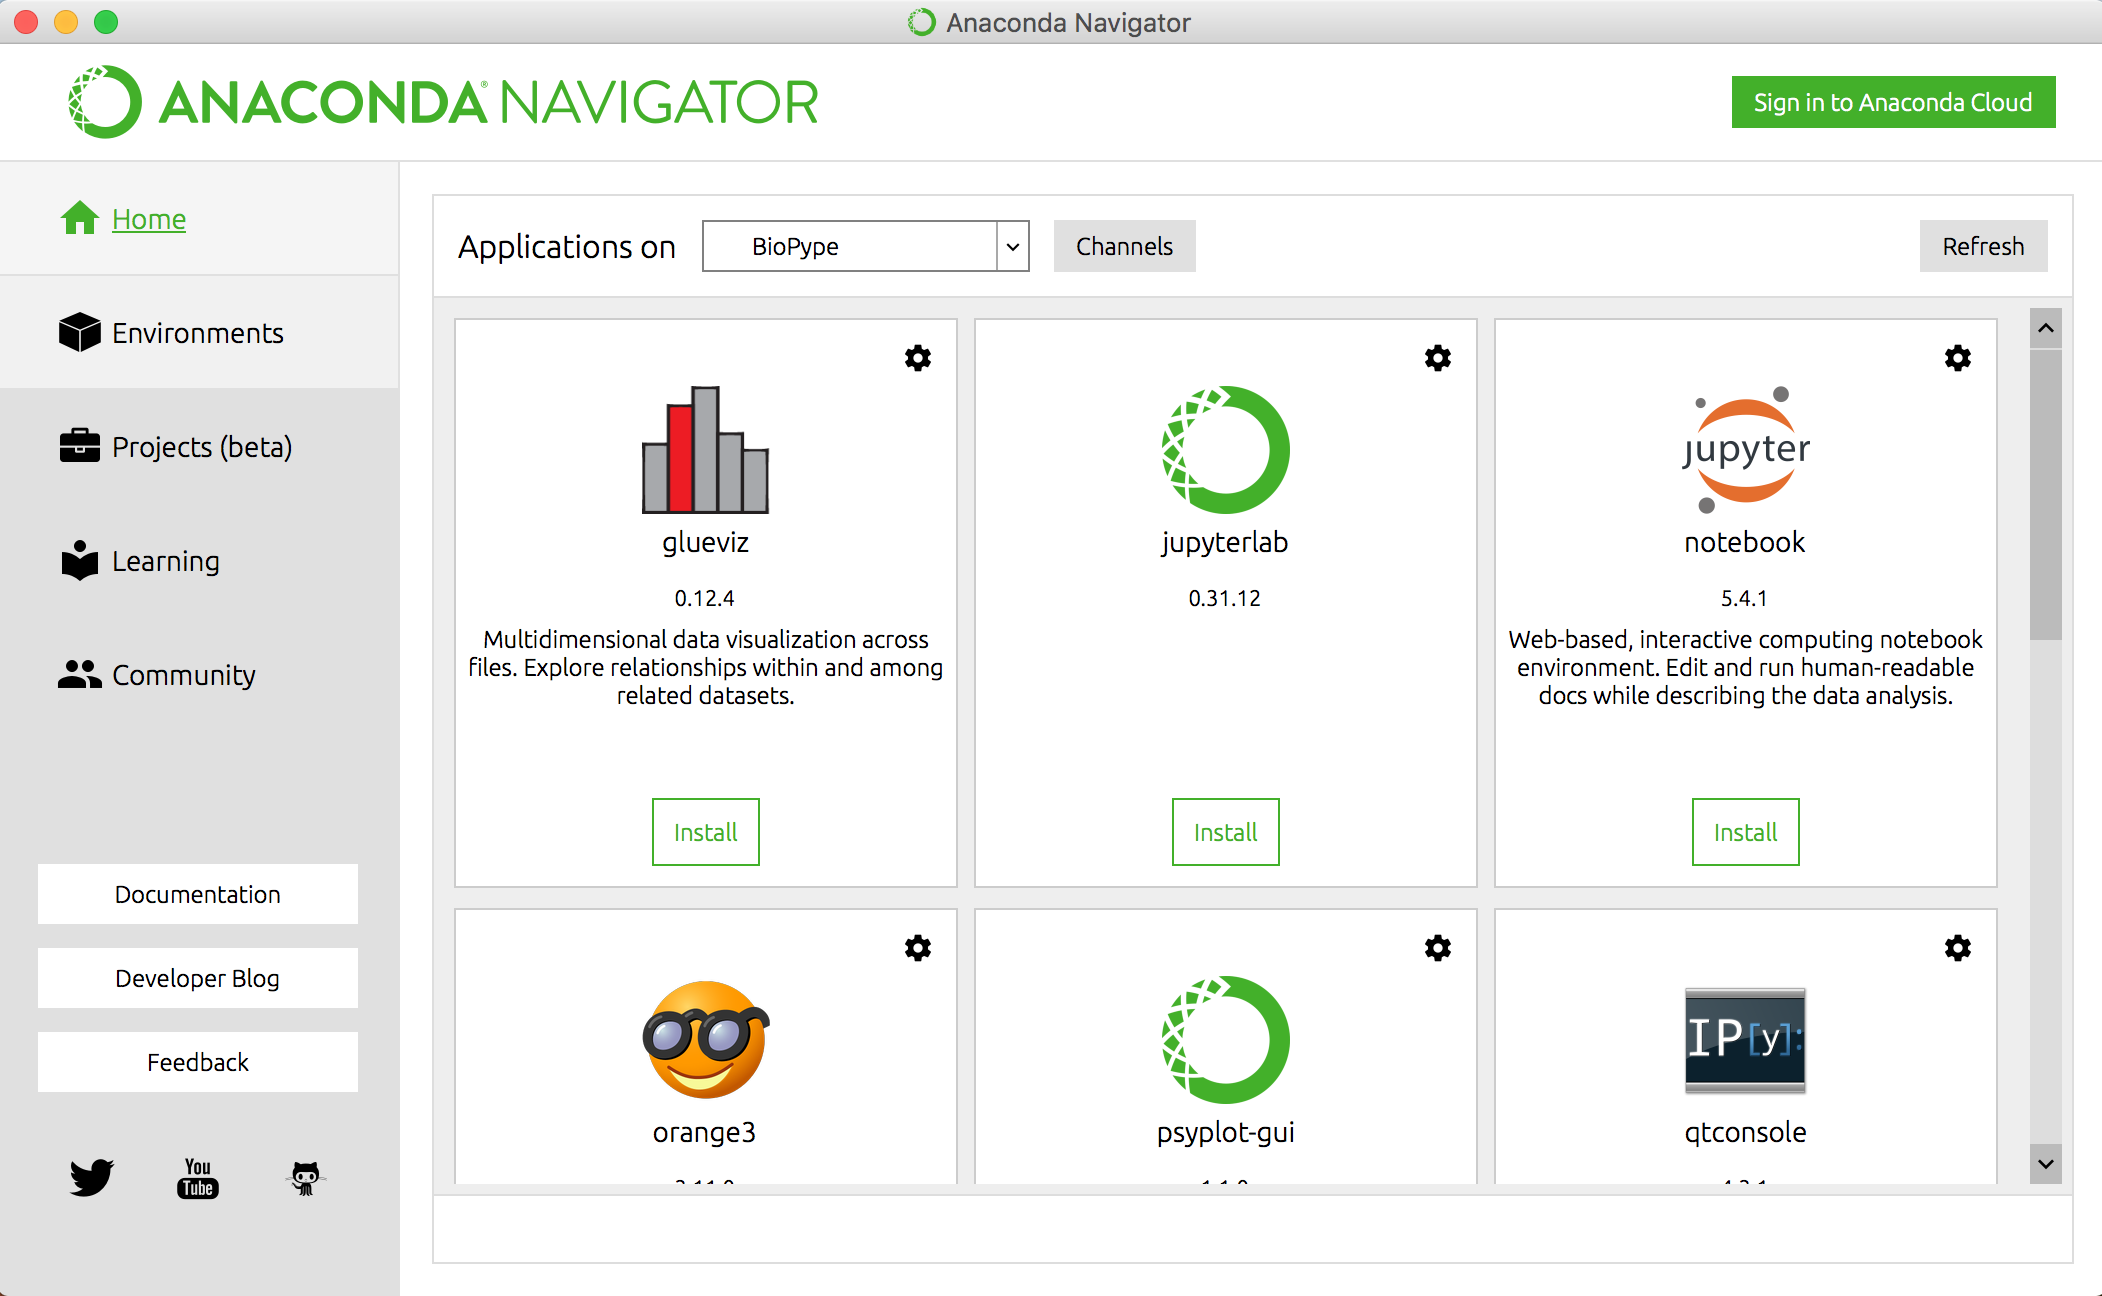
\includegraphics[width=12cm]{anaconda-nav-win}
        \caption{The window displayed to the user upon opening Anaconda-Navigator.}
        \label{anaconda-nav-win}
        \end{center}
    \end{figure}
    %
\end{enumerate}

\subsection{Create a New Virtual Environment}
    \todo[inline]{Write a blurb explaining the benefits of using a virtual environment.}
    \todo[inline]{Link to resource for further reading on virtual environments}
    \marginlabel{Make sure the computer has an internet connection while completing this section, otherwise Anaconda will not let you create a virtual environment.}
    \begin{enumerate}
        \item On the left side of the Anaconda-Navigator window, click on the tab labeled \textbf{Environments}. (Figure \ref{anaconda-env-win}) 
        %
        \begin{figure}
            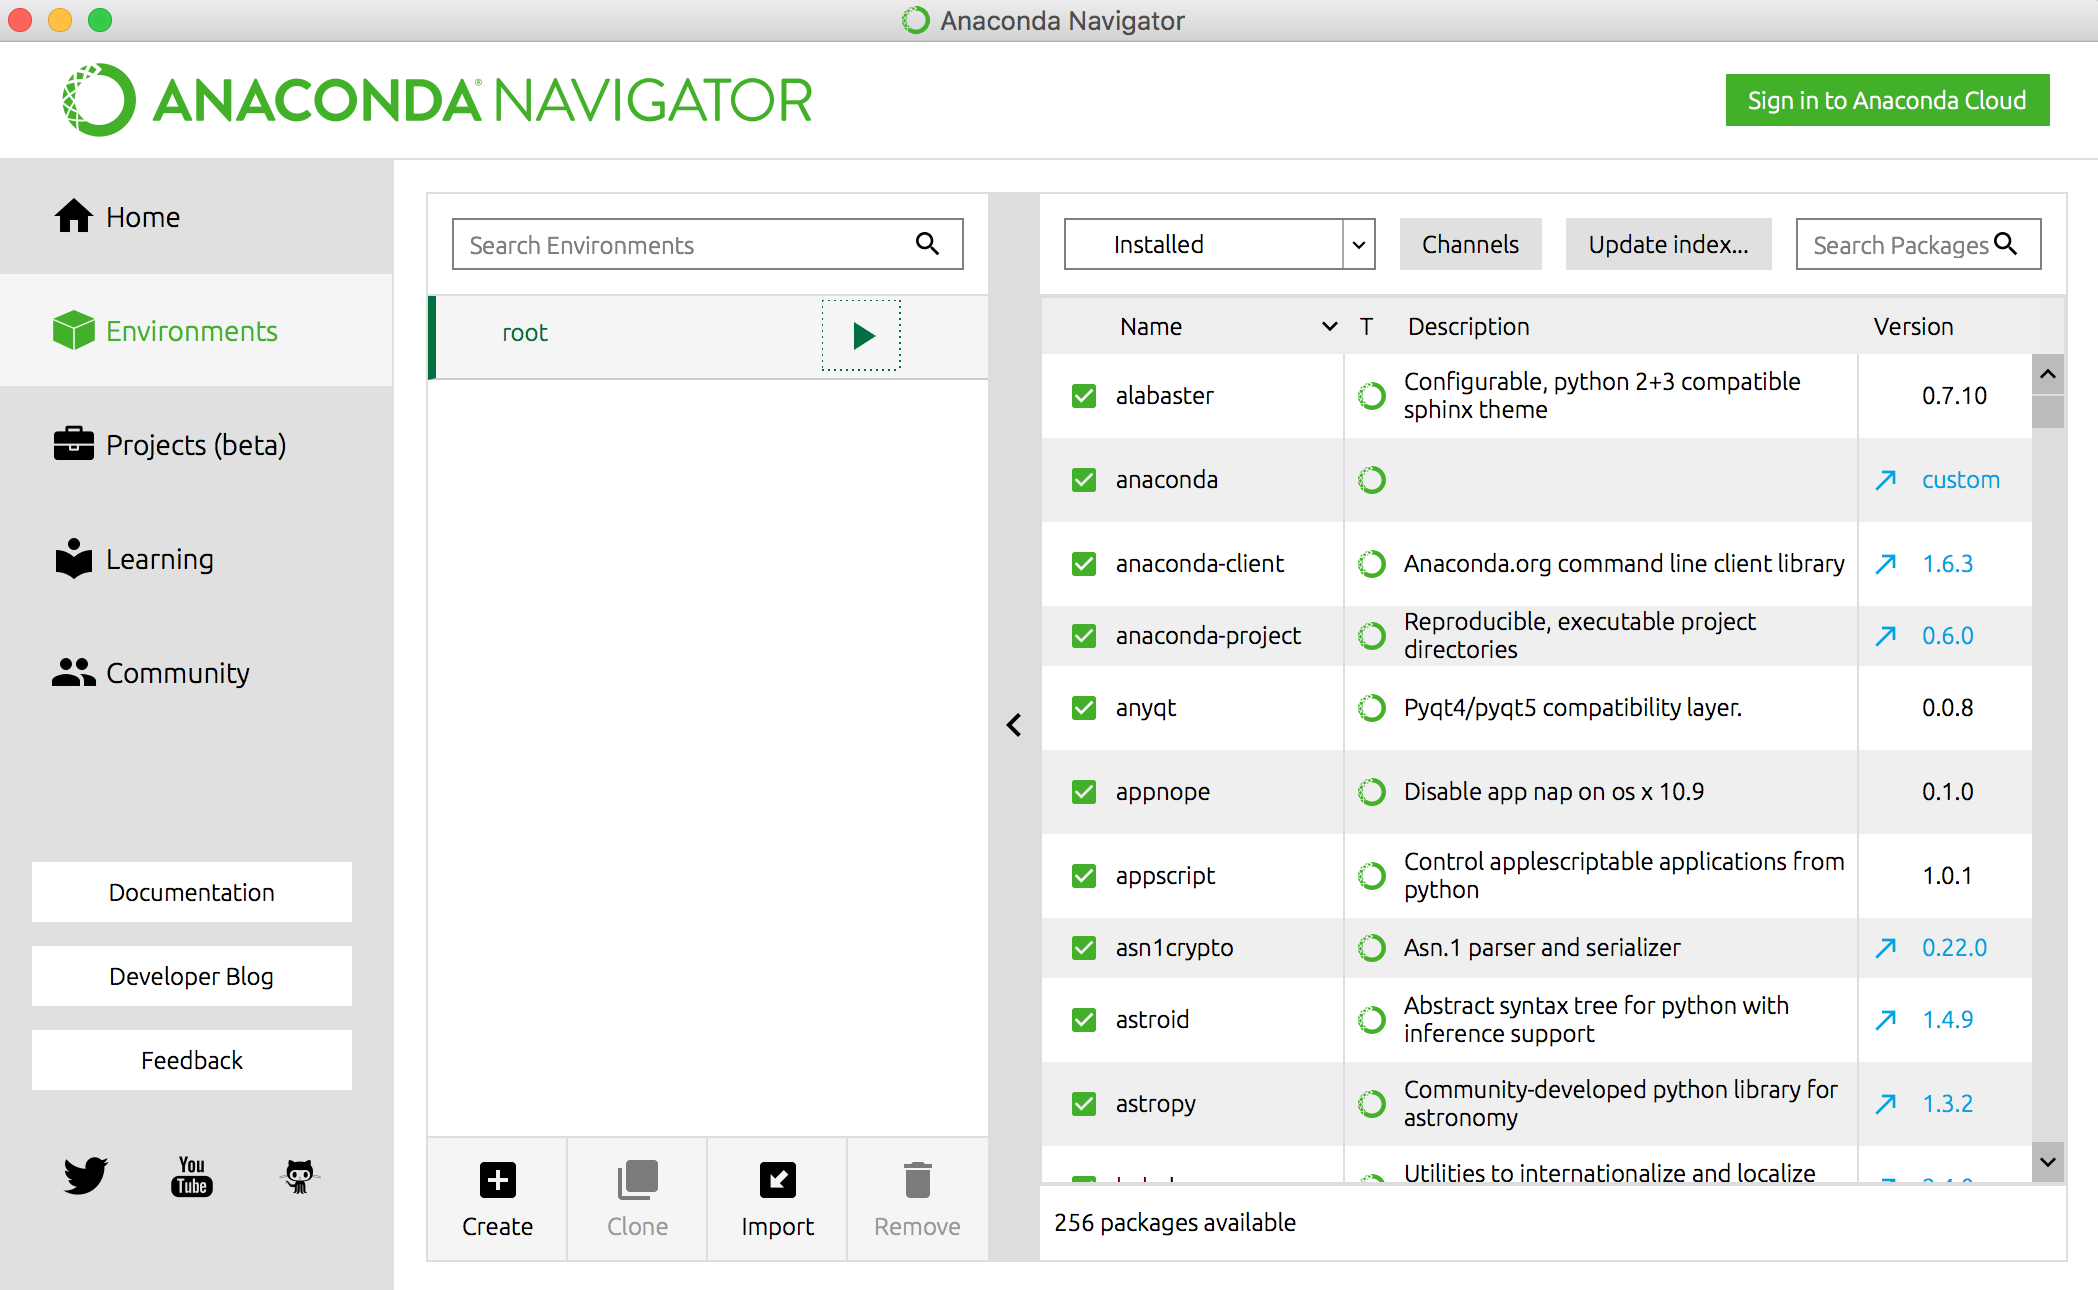
\includegraphics[width=12cm]{anaconda-env-win}
            \caption{The Environments window of the Anaconda-Navigator.}
            \label{anaconda-env-win}
        \end{figure}
        %
        \item Click the \textbf{Create} button on the bottom of the center panel. A new window titled "Create new environment" will appear. (Figure \ref{anaconda-create-new-env-win})
        %
        \begin{figure}[h]
            \begin{center}
            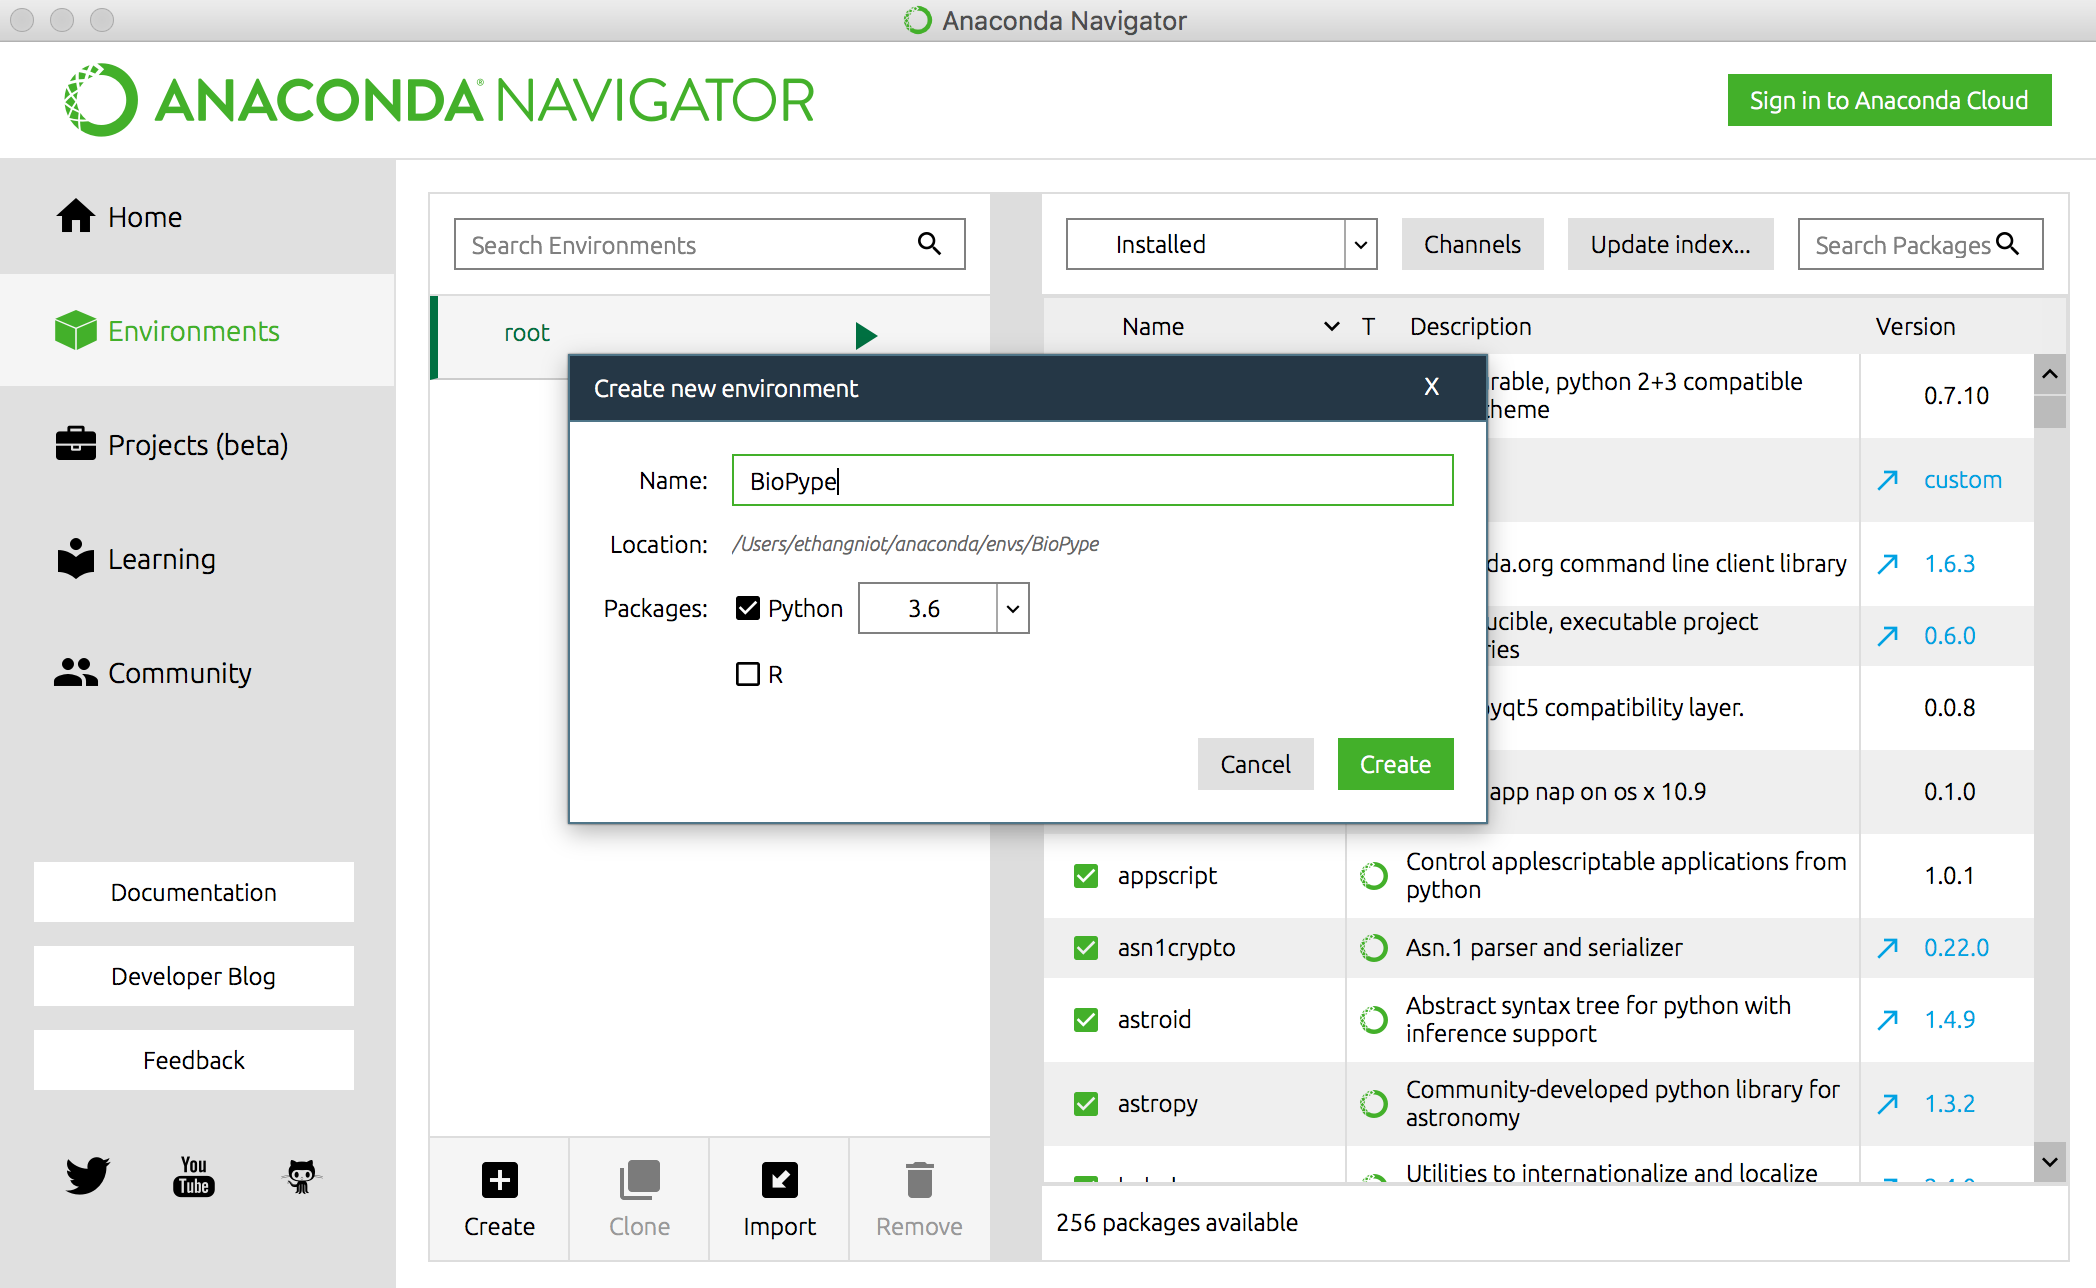
\includegraphics[width=12cm]{anaconda-create_new_env_win}
            \caption{The "Create new environment" window.}
            \label{anaconda-create-new-env-win}
            \end{center}
        \end{figure}
        %
        \item Enter a \textbf{Name} for the environment. You may choose any name you want, but for the sake of this tutorial we will name the new environment "BioPype".
        \item Select the box labeled \textbf{Python} next to the \textbf{Packages} heading.
        \item Choose a version of Python from the adjacent drop-down menu (Python 3.6 is the most current version at the time of this writing, but the packages we use require Python 3.5 so we chose \textbf{3.5}. If you are following the tutorial analysis in this manual, choose version 3.5).
        \item Click the \textbf{Create} button within the "Create new environment window".
    \end{enumerate}

\subsection{Install packages}
    \todo[inline]{Write blurb about what packages are.}
    \todo[inline]{Link to resource for further reading about packages.}
    \begin{enumerate}
        \item Change Anaconda's current environment from the \textbf{root} environment by selecting the \textbf{BioPype} tab in the middle panel of the Environments window.
        \item Click on the drop-down menu in the right-hand panel that says "Installed" and change it to "All".
        \item In the "Search Packages" box, enter "biopython". The search should return a package named "biopython". Select the checkbox to the left of the name. (Figure \ref{anaconda-search-pack})
        \begin{itemize}
            \item A pair of green and red boxes (reading "Apply" and "Clear", respectively) will appear in the bottom-right of the window once the package is selected. Do not click these just yet. 
    %
    \begin{figure}[hbtp]
        \begin{center}
        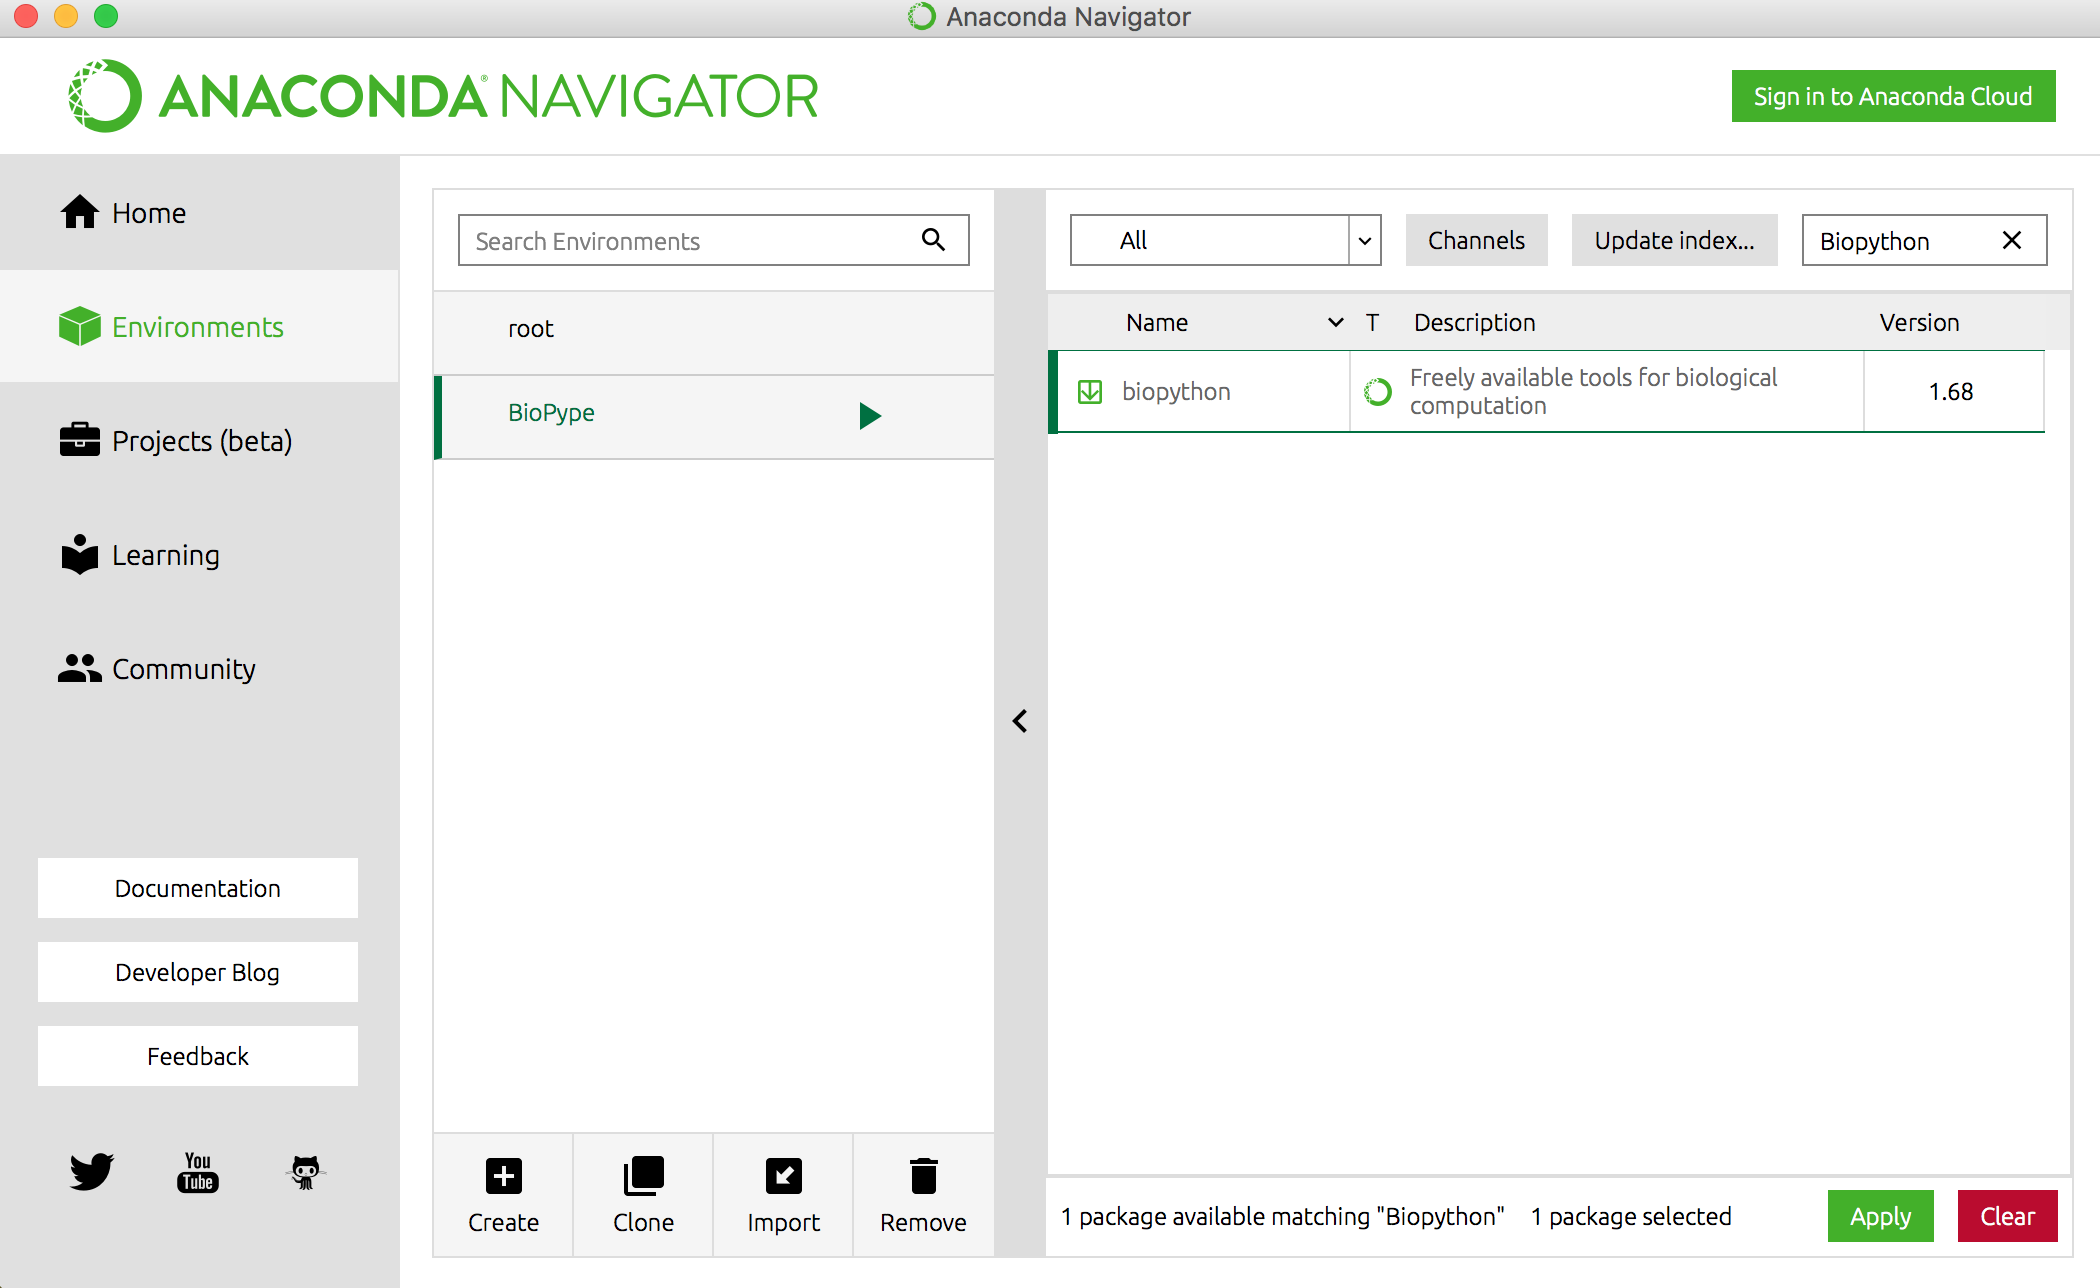
\includegraphics[width=12cm]{anaconda-search-pack}
        \caption{Searching for a package. When a package is selected, the checkbox next to the package's name will be green.}
        \label{anaconda-search-pack}
        \end{center}
    \end{figure}
    %
    \todo{Solve the issue with failing to center figures when they're on their own page}
        \end{itemize}
        \item Use the search bar to find and select the other packages listed in \autoref{tab:software}. Once all packages have been selected, click the green "Apply" button in the bottom right corner of the window, then select "Apply" again within the "Install Packages" window that appears. (Figure \ref{anaconda-install-pack}) Anaconda will now install the selected packages.
    %
    \begin{figure}[hbtp]
        \begin{center}
        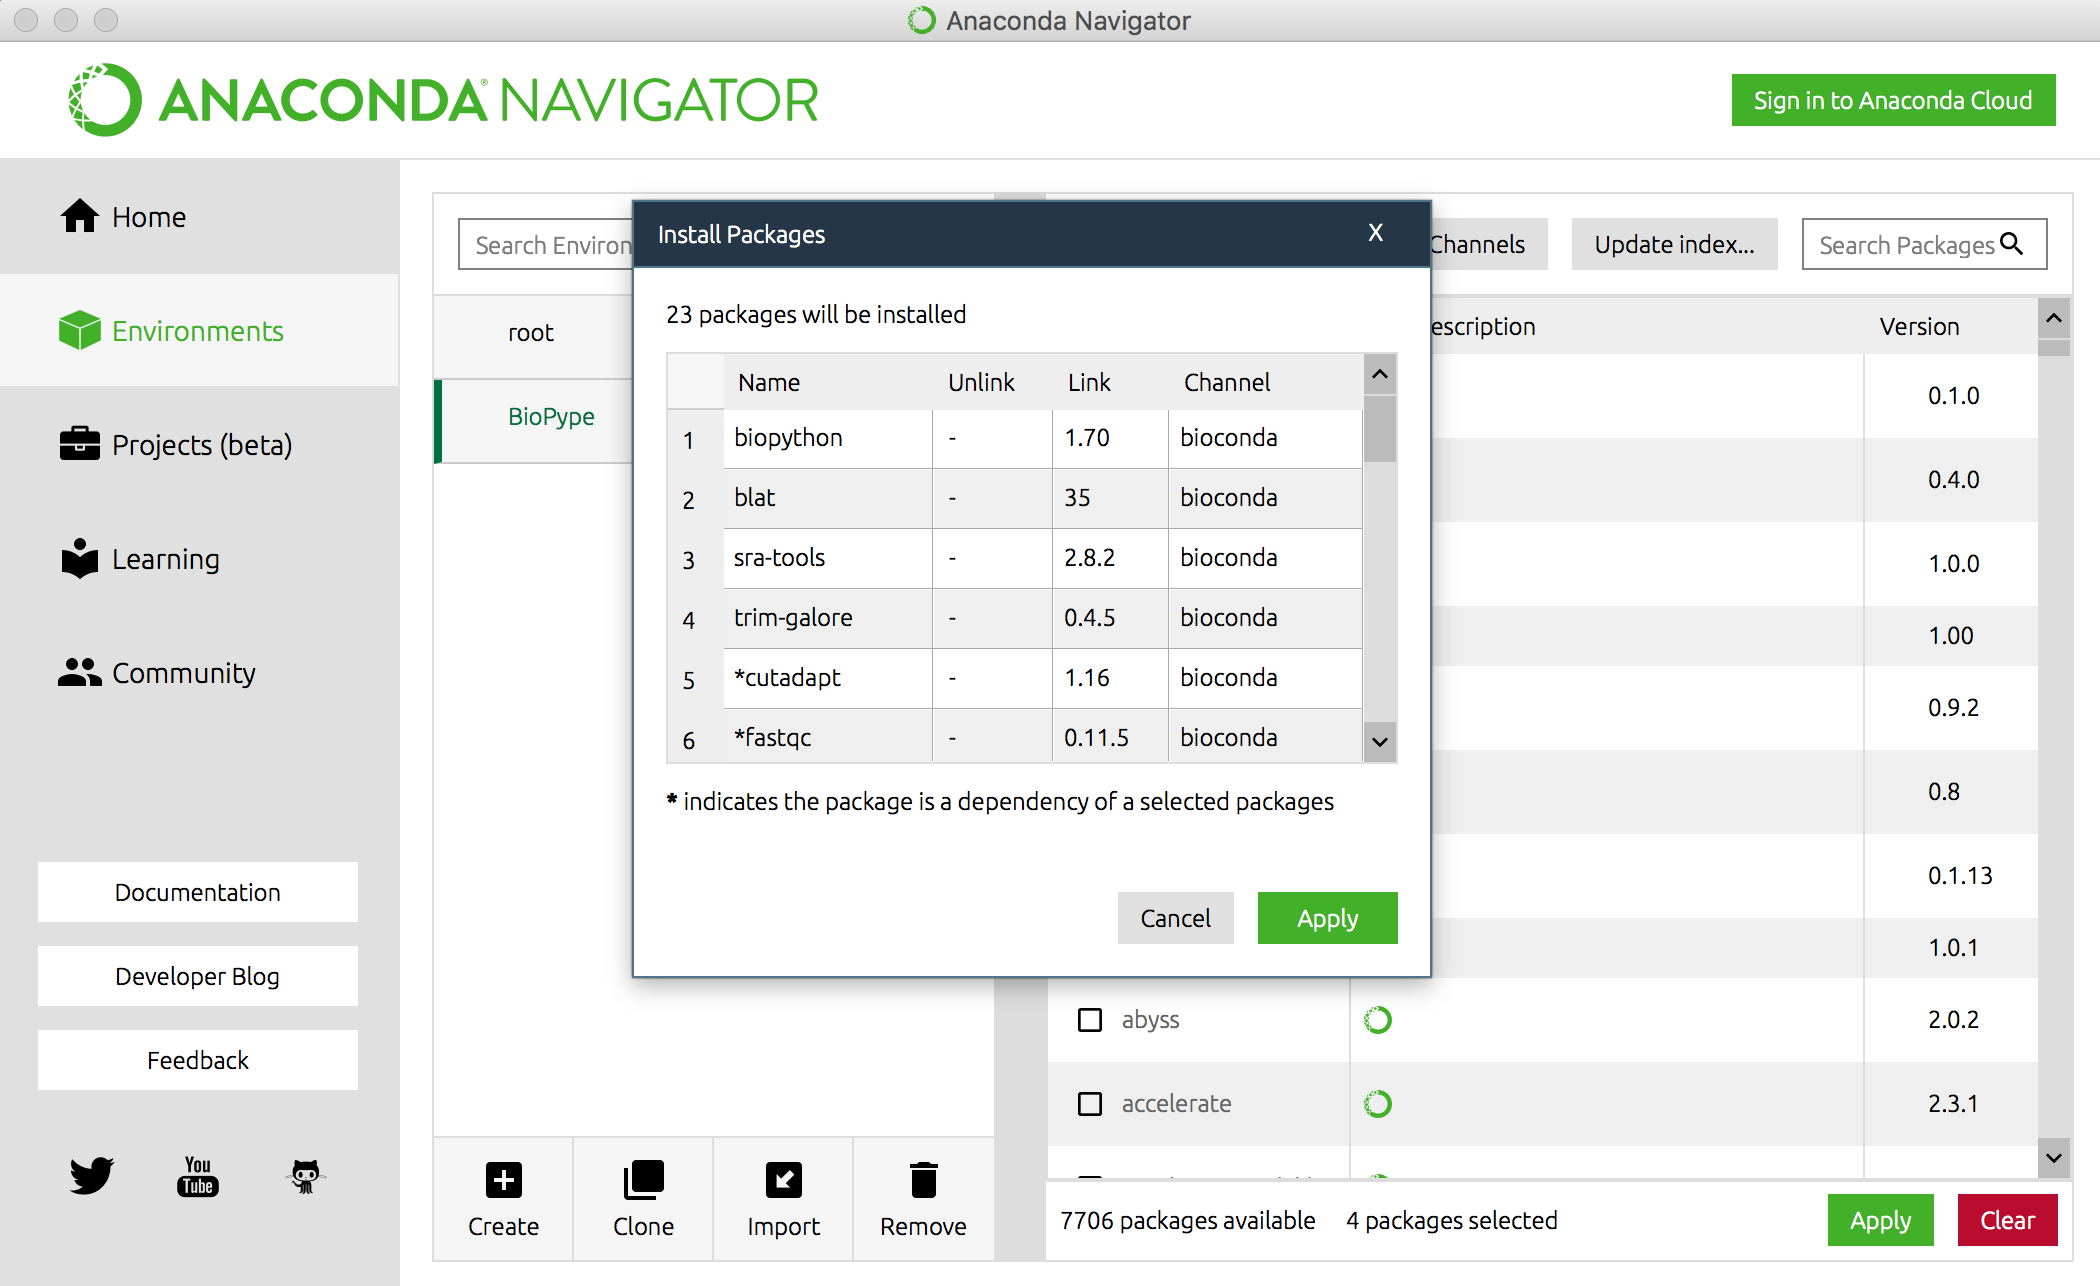
\includegraphics[width=12cm]{anaconda-install-pack}
        \caption{The window displaying the packages and dependencies that will be installed.}
        \label{anaconda-install-pack}
        \end{center}
    \end{figure}
    %
        \item \todo[inline]{Talk about setting up the sra-tools workspace (\url{https://trace.ncbi.nlm.nih.gov/Traces/sra/sra.cgi?view=toolkit_doc&f=std})}
        \item \todo[inline]{PYPIPER IS ONLY COMPATIBLE WITH MAC AND LINUX. Start by coding with just subprocess module commands. If the scripts work on Windows computers, then forget about using pypiper. But if the subprocess scripts don't work on windows, then we'll be developing exclusively for Mac anyways, so you could use pypiper without any worries. In that case, talk about installing pypiper here. OTHERWISE, delete this section.}
        \begin{enumerate}
            \item Open a terminal window in the BioPype environment by clicking the "play" button on the BioPype environment tab and then selecting "Open Terminal".
            \item Wait for the terminal window to finish opening. You'll know it's finished when you see \todo[inline]{show image of what the prompt looks like when it's done initializing.}
            \item Install \textbf{pypiper} by typing the following at the command prompt, followed by pressing return/enter:
            %
            \begin{lstlisting} [language=Python]
                pip install --user pypiper
            \end{lstlisting}
            %
            \item Check that the package was installed correctly by executing the following in the command prompt:
            %
            \begin{lstlisting} [language=Python]
                conda list
            \end{lstlisting}
            %
            This will generate a list of all the packages installed in the current environment. If you see the \textbf{pypiper} package listed, the installation was successful and you may skip the rest of this section. If not, proceed with the following steps.
            \item Execute the install command from step (c) again. This time, the Terminal should return a message similar to the one displayed in \todo[inline]{Reference the figure pypiper-already-installed}. The line that reads "Requirement already satisfied: pypiper in ...." tells us the location where the package was (incorrectly) installed. 
            \missingfigure{pypiper-already-installed}
            \item Open a Terminal window, and navigate to the location indicated by the message from the previous step. For my example, I need to start at my home directory and walk through the following folders: .local | lib | python3.6 | site-packages. 
            \begin{itemize}
                \item The folders along the path to the pypiper installation may be hidden. On a Mac, these hidden folders are preceded by a "." If the path to the pypiper installation includes hidden locations, reveal them by pressing "Cmd + Shift + ." in the Finder window.
            \item Once you find the site-packages folder containing two pypiper folders \todo[inline]{reference figure pypiper-wrong-location}, copy those folders and their contents and paste them into the ~/anaconda/envs/BioPype/lib/python3.6/site-packages directory. The package should now be installed correctly. \missingfigure{pypiper-wrong-location} 
            \marginlabel{}
            \end{itemize}
        \end{enumerate}    
    \end{enumerate}

\subsection{Integrated Development Environment (IDE)}
\todo[inline]{Talk about choosing between PyCharm and other options}
%
\subsection{PATH}
\todo[inline]{(Talk about putting all the tools in the same path/directory)}
\section{Analysis Pipeline}
(Use figures to illustrate the stages of the pipeline)
